% Options for packages loaded elsewhere
% Options for packages loaded elsewhere
\PassOptionsToPackage{unicode}{hyperref}
\PassOptionsToPackage{hyphens}{url}
\PassOptionsToPackage{dvipsnames,svgnames,x11names}{xcolor}
%
\documentclass[
  letterpaper,
  DIV=11,
  numbers=noendperiod]{scrartcl}
\usepackage{xcolor}
\usepackage{amsmath,amssymb}
\setcounter{secnumdepth}{-\maxdimen} % remove section numbering
\usepackage{iftex}
\ifPDFTeX
  \usepackage[T1]{fontenc}
  \usepackage[utf8]{inputenc}
  \usepackage{textcomp} % provide euro and other symbols
\else % if luatex or xetex
  \usepackage{unicode-math} % this also loads fontspec
  \defaultfontfeatures{Scale=MatchLowercase}
  \defaultfontfeatures[\rmfamily]{Ligatures=TeX,Scale=1}
\fi
\usepackage{lmodern}
\ifPDFTeX\else
  % xetex/luatex font selection
\fi
% Use upquote if available, for straight quotes in verbatim environments
\IfFileExists{upquote.sty}{\usepackage{upquote}}{}
\IfFileExists{microtype.sty}{% use microtype if available
  \usepackage[]{microtype}
  \UseMicrotypeSet[protrusion]{basicmath} % disable protrusion for tt fonts
}{}
\makeatletter
\@ifundefined{KOMAClassName}{% if non-KOMA class
  \IfFileExists{parskip.sty}{%
    \usepackage{parskip}
  }{% else
    \setlength{\parindent}{0pt}
    \setlength{\parskip}{6pt plus 2pt minus 1pt}}
}{% if KOMA class
  \KOMAoptions{parskip=half}}
\makeatother
% Make \paragraph and \subparagraph free-standing
\makeatletter
\ifx\paragraph\undefined\else
  \let\oldparagraph\paragraph
  \renewcommand{\paragraph}{
    \@ifstar
      \xxxParagraphStar
      \xxxParagraphNoStar
  }
  \newcommand{\xxxParagraphStar}[1]{\oldparagraph*{#1}\mbox{}}
  \newcommand{\xxxParagraphNoStar}[1]{\oldparagraph{#1}\mbox{}}
\fi
\ifx\subparagraph\undefined\else
  \let\oldsubparagraph\subparagraph
  \renewcommand{\subparagraph}{
    \@ifstar
      \xxxSubParagraphStar
      \xxxSubParagraphNoStar
  }
  \newcommand{\xxxSubParagraphStar}[1]{\oldsubparagraph*{#1}\mbox{}}
  \newcommand{\xxxSubParagraphNoStar}[1]{\oldsubparagraph{#1}\mbox{}}
\fi
\makeatother

\usepackage{color}
\usepackage{fancyvrb}
\newcommand{\VerbBar}{|}
\newcommand{\VERB}{\Verb[commandchars=\\\{\}]}
\DefineVerbatimEnvironment{Highlighting}{Verbatim}{commandchars=\\\{\}}
% Add ',fontsize=\small' for more characters per line
\usepackage{framed}
\definecolor{shadecolor}{RGB}{241,243,245}
\newenvironment{Shaded}{\begin{snugshade}}{\end{snugshade}}
\newcommand{\AlertTok}[1]{\textcolor[rgb]{0.68,0.00,0.00}{#1}}
\newcommand{\AnnotationTok}[1]{\textcolor[rgb]{0.37,0.37,0.37}{#1}}
\newcommand{\AttributeTok}[1]{\textcolor[rgb]{0.40,0.45,0.13}{#1}}
\newcommand{\BaseNTok}[1]{\textcolor[rgb]{0.68,0.00,0.00}{#1}}
\newcommand{\BuiltInTok}[1]{\textcolor[rgb]{0.00,0.23,0.31}{#1}}
\newcommand{\CharTok}[1]{\textcolor[rgb]{0.13,0.47,0.30}{#1}}
\newcommand{\CommentTok}[1]{\textcolor[rgb]{0.37,0.37,0.37}{#1}}
\newcommand{\CommentVarTok}[1]{\textcolor[rgb]{0.37,0.37,0.37}{\textit{#1}}}
\newcommand{\ConstantTok}[1]{\textcolor[rgb]{0.56,0.35,0.01}{#1}}
\newcommand{\ControlFlowTok}[1]{\textcolor[rgb]{0.00,0.23,0.31}{\textbf{#1}}}
\newcommand{\DataTypeTok}[1]{\textcolor[rgb]{0.68,0.00,0.00}{#1}}
\newcommand{\DecValTok}[1]{\textcolor[rgb]{0.68,0.00,0.00}{#1}}
\newcommand{\DocumentationTok}[1]{\textcolor[rgb]{0.37,0.37,0.37}{\textit{#1}}}
\newcommand{\ErrorTok}[1]{\textcolor[rgb]{0.68,0.00,0.00}{#1}}
\newcommand{\ExtensionTok}[1]{\textcolor[rgb]{0.00,0.23,0.31}{#1}}
\newcommand{\FloatTok}[1]{\textcolor[rgb]{0.68,0.00,0.00}{#1}}
\newcommand{\FunctionTok}[1]{\textcolor[rgb]{0.28,0.35,0.67}{#1}}
\newcommand{\ImportTok}[1]{\textcolor[rgb]{0.00,0.46,0.62}{#1}}
\newcommand{\InformationTok}[1]{\textcolor[rgb]{0.37,0.37,0.37}{#1}}
\newcommand{\KeywordTok}[1]{\textcolor[rgb]{0.00,0.23,0.31}{\textbf{#1}}}
\newcommand{\NormalTok}[1]{\textcolor[rgb]{0.00,0.23,0.31}{#1}}
\newcommand{\OperatorTok}[1]{\textcolor[rgb]{0.37,0.37,0.37}{#1}}
\newcommand{\OtherTok}[1]{\textcolor[rgb]{0.00,0.23,0.31}{#1}}
\newcommand{\PreprocessorTok}[1]{\textcolor[rgb]{0.68,0.00,0.00}{#1}}
\newcommand{\RegionMarkerTok}[1]{\textcolor[rgb]{0.00,0.23,0.31}{#1}}
\newcommand{\SpecialCharTok}[1]{\textcolor[rgb]{0.37,0.37,0.37}{#1}}
\newcommand{\SpecialStringTok}[1]{\textcolor[rgb]{0.13,0.47,0.30}{#1}}
\newcommand{\StringTok}[1]{\textcolor[rgb]{0.13,0.47,0.30}{#1}}
\newcommand{\VariableTok}[1]{\textcolor[rgb]{0.07,0.07,0.07}{#1}}
\newcommand{\VerbatimStringTok}[1]{\textcolor[rgb]{0.13,0.47,0.30}{#1}}
\newcommand{\WarningTok}[1]{\textcolor[rgb]{0.37,0.37,0.37}{\textit{#1}}}

\usepackage{longtable,booktabs,array}
\usepackage{calc} % for calculating minipage widths
% Correct order of tables after \paragraph or \subparagraph
\usepackage{etoolbox}
\makeatletter
\patchcmd\longtable{\par}{\if@noskipsec\mbox{}\fi\par}{}{}
\makeatother
% Allow footnotes in longtable head/foot
\IfFileExists{footnotehyper.sty}{\usepackage{footnotehyper}}{\usepackage{footnote}}
\makesavenoteenv{longtable}
\usepackage{graphicx}
\makeatletter
\newsavebox\pandoc@box
\newcommand*\pandocbounded[1]{% scales image to fit in text height/width
  \sbox\pandoc@box{#1}%
  \Gscale@div\@tempa{\textheight}{\dimexpr\ht\pandoc@box+\dp\pandoc@box\relax}%
  \Gscale@div\@tempb{\linewidth}{\wd\pandoc@box}%
  \ifdim\@tempb\p@<\@tempa\p@\let\@tempa\@tempb\fi% select the smaller of both
  \ifdim\@tempa\p@<\p@\scalebox{\@tempa}{\usebox\pandoc@box}%
  \else\usebox{\pandoc@box}%
  \fi%
}
% Set default figure placement to htbp
\def\fps@figure{htbp}
\makeatother





\setlength{\emergencystretch}{3em} % prevent overfull lines

\providecommand{\tightlist}{%
  \setlength{\itemsep}{0pt}\setlength{\parskip}{0pt}}



 


\KOMAoption{captions}{tableheading}
\makeatletter
\@ifpackageloaded{caption}{}{\usepackage{caption}}
\AtBeginDocument{%
\ifdefined\contentsname
  \renewcommand*\contentsname{Table of contents}
\else
  \newcommand\contentsname{Table of contents}
\fi
\ifdefined\listfigurename
  \renewcommand*\listfigurename{List of Figures}
\else
  \newcommand\listfigurename{List of Figures}
\fi
\ifdefined\listtablename
  \renewcommand*\listtablename{List of Tables}
\else
  \newcommand\listtablename{List of Tables}
\fi
\ifdefined\figurename
  \renewcommand*\figurename{Figure}
\else
  \newcommand\figurename{Figure}
\fi
\ifdefined\tablename
  \renewcommand*\tablename{Table}
\else
  \newcommand\tablename{Table}
\fi
}
\@ifpackageloaded{float}{}{\usepackage{float}}
\floatstyle{ruled}
\@ifundefined{c@chapter}{\newfloat{codelisting}{h}{lop}}{\newfloat{codelisting}{h}{lop}[chapter]}
\floatname{codelisting}{Listing}
\newcommand*\listoflistings{\listof{codelisting}{List of Listings}}
\makeatother
\makeatletter
\makeatother
\makeatletter
\@ifpackageloaded{caption}{}{\usepackage{caption}}
\@ifpackageloaded{subcaption}{}{\usepackage{subcaption}}
\makeatother
\usepackage{bookmark}
\IfFileExists{xurl.sty}{\usepackage{xurl}}{} % add URL line breaks if available
\urlstyle{same}
\hypersetup{
  pdftitle={Coral\_arcGIS\_analysis},
  pdfauthor={Jessica Riker},
  colorlinks=true,
  linkcolor={blue},
  filecolor={Maroon},
  citecolor={Blue},
  urlcolor={Blue},
  pdfcreator={LaTeX via pandoc}}


\title{Coral\_arcGIS\_analysis}
\author{Jessica Riker}
\date{}
\begin{document}
\maketitle


\begin{Shaded}
\begin{Highlighting}[]
\CommentTok{\# setup and add packages}
\CommentTok{\#| label: setup}
\CommentTok{\#| include: false}
\FunctionTok{library}\NormalTok{(tidyverse)}
\end{Highlighting}
\end{Shaded}

\begin{verbatim}
-- Attaching core tidyverse packages ------------------------ tidyverse 2.0.0 --
v dplyr     1.2.1     v readr     2.2.0
v forcats   1.0.1     v stringr   1.6.0
v ggplot2   4.0.3     v tibble    3.3.1
v lubridate 1.9.4     v tidyr     1.3.2
v purrr     1.2.1     
-- Conflicts ------------------------------------------ tidyverse_conflicts() --
x dplyr::filter() masks stats::filter()
x dplyr::lag()    masks stats::lag()
i Use the conflicted package (<http://conflicted.r-lib.org/>) to force all conflicts to become errors
\end{verbatim}

\begin{Shaded}
\begin{Highlighting}[]
\FunctionTok{library}\NormalTok{(readxl)}
\FunctionTok{library}\NormalTok{(scales)}
\end{Highlighting}
\end{Shaded}

\begin{verbatim}

Attaching package: 'scales'

The following object is masked from 'package:purrr':

    discard

The following object is masked from 'package:readr':

    col_factor
\end{verbatim}

\begin{Shaded}
\begin{Highlighting}[]
\CommentTok{\# inspect csvs for nearest neighbor, ripleys k, and colony attributes}
\FunctionTok{glimpse}\NormalTok{(}\FunctionTok{read\_csv}\NormalTok{(}\StringTok{"data/Nearest Neighbor/BA\_NearSameTaxa.csv"}\NormalTok{, }\AttributeTok{show\_col\_types =} \ConstantTok{FALSE}\NormalTok{))}
\end{Highlighting}
\end{Shaded}

\begin{verbatim}
Rows: 2,120
Columns: 4
$ OBJECTID  <dbl> 0, 0, 0, 0, 0, 0, 0, 0, 0, 0, 0, 0, 0, 0, 0, 0, 0, 0, 0, 0, ~
$ IN_FID    <dbl> 1, 2, 3, 4, 5, 6, 7, 8, 9, 10, 11, 12, 13, 14, 15, 16, 17, 1~
$ NEAR_FID  <dbl> 234, 236, 13, 268, 6, 5, 123, 1098, 126, 129, 130, 101, 3, 5~
$ NEAR_DIST <dbl> 0.44657678, 0.56644099, 0.11854286, 0.28047894, 0.01751142, ~
\end{verbatim}

\begin{Shaded}
\begin{Highlighting}[]
\FunctionTok{glimpse}\NormalTok{(}\FunctionTok{read\_csv}\NormalTok{(}\StringTok{"data/Nearest Neighbor/BA\_neardifftaxa.csv"}\NormalTok{, }\AttributeTok{show\_col\_types =} \ConstantTok{FALSE}\NormalTok{))}
\end{Highlighting}
\end{Shaded}

\begin{verbatim}
Rows: 10,625
Columns: 10
$ OBJECTID     <dbl> 0, 0, 0, 0, 0, 0, 0, 0, 0, 0, 0, 0, 0, 0, 0, 0, 0, 0, 0, ~
$ IN_FID       <dbl> 1, 1, 1, 1, 1, 2, 2, 2, 2, 2, 3, 3, 3, 3, 3, 4, 4, 4, 4, ~
$ NEAR_FID     <dbl> 2, 13, 3, 234, 235, 1, 3, 13, 234, 235, 4, 2, 1, 13, 54, ~
$ NEAR_DIST    <dbl> 0.00000000, 0.00000000, 0.09984388, 0.44657678, 0.5203617~
$ NEAR_RANK    <dbl> 1, 1, 2, 3, 4, 1, 2, 3, 4, 5, 1, 2, 3, 4, 5, 1, 2, 3, 4, ~
$ CLEANEDPRE   <chr> "G_POR", "G_POR", "G_POR", "G_POR", "G_POR", "SCM", "SCM"~
$ SHAPE_AREA   <dbl> 0.03860705, 0.03860705, 0.03860705, 0.03860705, 0.0386070~
$ IN_TAXA      <dbl> 1, 1, 1, 1, 1, 2, 2, 2, 2, 2, 3, 3, 3, 3, 3, 4, 4, 4, 4, ~
$ IN_AREA      <dbl> 0.03860705, 0.03860705, 0.03860705, 0.03860705, 0.0386070~
$ CLEANEDPRE_1 <chr> "SCM", "ACO_OTH", "ACO_OTH", "G_POR", "ENC_OTH_MON", "G_P~
\end{verbatim}

\begin{Shaded}
\begin{Highlighting}[]
\FunctionTok{glimpse}\NormalTok{(}\FunctionTok{read\_csv}\NormalTok{(}\StringTok{"data/Ripleys K/BA\_Ripley\textquotesingle{}s.csv"}\NormalTok{, }\AttributeTok{show\_col\_types =} \ConstantTok{FALSE}\NormalTok{))}
\end{Highlighting}
\end{Shaded}

\begin{verbatim}
Rows: 10
Columns: 5
$ ExpectedK <dbl> 0.3284122, 0.6568244, 0.9852366, 1.3136489, 1.6420611, 1.970~
$ ObservedK <dbl> 0.5407383, 0.9561914, 1.3260555, 1.6826875, 2.0369613, 2.389~
$ DiffK     <dbl> 0.2123261, 0.2993669, 0.3408188, 0.3690386, 0.3949002, 0.418~
$ LwConfEnv <dbl> 0.3247105, 0.6535698, 0.9787515, 1.3040319, 1.6254245, 1.942~
$ HiConfEnv <dbl> 0.3338219, 0.6632247, 0.9891258, 1.3148304, 1.6409551, 1.961~
\end{verbatim}

\begin{Shaded}
\begin{Highlighting}[]
\FunctionTok{glimpse}\NormalTok{(}\FunctionTok{read\_csv}\NormalTok{(}\StringTok{"data/Colony Attributes/BA\_attributes.csv"}\NormalTok{, }\AttributeTok{show\_col\_types =} \ConstantTok{FALSE}\NormalTok{))}
\end{Highlighting}
\end{Shaded}

\begin{verbatim}
Rows: 64
Columns: 5
$ CleanedPre       <chr> NA, "AAC", "AC_Bran_OTH", "ACD", "ACF", "ACO_OTH", "A~
$ SUM_Shape_Area   <dbl> 0.07491277, 0.21462917, 0.45891160, 0.43168540, 0.025~
$ SUM_Shape_Length <dbl> 2.8265592, 6.3538245, 10.1801777, 18.9733928, 2.13575~
$ Shape_Length     <dbl> 2.8254705, 6.3008759, 9.7220041, 14.7293011, 1.990693~
$ Shape_Area       <dbl> 0.07491903, 0.21457074, 0.45889337, 0.43186022, 0.025~
\end{verbatim}

\begin{Shaded}
\begin{Highlighting}[]
\CommentTok{\# FR4 / FR / FA4 files}
\FunctionTok{glimpse}\NormalTok{(}\FunctionTok{read\_csv}\NormalTok{(}\StringTok{"data/Nearest Neighbor/FR4\_NearSameTaxa.csv"}\NormalTok{, }\AttributeTok{show\_col\_types =} \ConstantTok{FALSE}\NormalTok{))}
\end{Highlighting}
\end{Shaded}

\begin{verbatim}
Rows: 1,843
Columns: 4
$ OBJECTID  <dbl> 0, 0, 0, 0, 0, 0, 0, 0, 0, 0, 0, 0, 0, 0, 0, 0, 0, 0, 0, 0, ~
$ IN_FID    <dbl> 1, 2, 7, 8, 9, 10, 11, 12, 13, 36, 53, 55, 60, 62, 63, 64, 6~
$ NEAR_FID  <dbl> 2, 976, 8, 7, 8, 8, 12, 11, 4160, 8629, 274, 8638, 1081, 116~
$ NEAR_DIST <dbl> 0.08634611, 0.00000000, 0.00000000, 0.00000000, 0.00000000, ~
\end{verbatim}

\begin{Shaded}
\begin{Highlighting}[]
\FunctionTok{glimpse}\NormalTok{(}\FunctionTok{read\_csv}\NormalTok{(}\StringTok{"data/Nearest Neighbor/FR4\_neardifftaxa.csv"}\NormalTok{, }\AttributeTok{show\_col\_types =} \ConstantTok{FALSE}\NormalTok{))}
\end{Highlighting}
\end{Shaded}

\begin{verbatim}
Rows: 9,220
Columns: 12
$ OBJECTID     <dbl> 0, 0, 0, 0, 0, 0, 0, 0, 0, 0, 0, 0, 0, 0, 0, 0, 0, 0, 0, ~
$ IN_FID       <dbl> 1, 1, 1, 1, 1, 2, 2, 2, 2, 2, 7, 7, 7, 7, 7, 8, 8, 8, 8, ~
$ NEAR_FID     <dbl> 200, 8652, 8650, 2, 896, 200, 976, 1408, 977, 2405, 8, 41~
$ NEAR_DIST    <dbl> 0.000000000, 0.000000000, 0.048804302, 0.086346106, 0.098~
$ NEAR_RANK    <dbl> 1, 1, 2, 3, 4, 1, 1, 1, 2, 3, 1, 1, 1, 1, 2, 1, 1, 1, 1, ~
$ CLEANEDPRE   <lgl> NA, NA, NA, NA, NA, NA, NA, NA, NA, NA, NA, NA, NA, NA, N~
$ SHAPE_AREA   <dbl> 0, 0, 0, 0, 0, 0, 0, 0, 0, 0, 0, 0, 0, 0, 0, 0, 0, 0, 0, ~
$ PRED_DESC_   <chr> "SCM", "SCM", "SCM", "SCM", "SCM", "SCM", "SCM", "SCM", "~
$ SHAPE_AREA_1 <dbl> 0.102789265, 0.102789265, 0.102789265, 0.102789265, 0.102~
$ IN_TAXA      <dbl> 1, 1, 1, 1, 1, 2, 2, 2, 2, 2, 7, 7, 7, 7, 7, 8, 8, 8, 8, ~
$ IN_AREA      <dbl> 0.102789265, 0.102789265, 0.102789265, 0.102789265, 0.102~
$ PRED_DESC1   <chr> "ACS", "G_LOB", "ACO_OTH", "SCM", "ACS", "ACS", "SCM", "S~
\end{verbatim}

\begin{Shaded}
\begin{Highlighting}[]
\FunctionTok{glimpse}\NormalTok{(}\FunctionTok{read\_csv}\NormalTok{(}\StringTok{"data/Ripleys K/FA4\_Ripley\textquotesingle{}s.csv"}\NormalTok{, }\AttributeTok{show\_col\_types =} \ConstantTok{FALSE}\NormalTok{))}
\end{Highlighting}
\end{Shaded}

\begin{verbatim}
Rows: 10
Columns: 5
$ ExpectedK <dbl> 0.3202802, 0.6405604, 0.9608407, 1.2811209, 1.6014011, 1.921~
$ ObservedK <dbl> 0.4519440, 0.8014755, 1.1350570, 1.4678398, 1.7870794, 2.101~
$ DiffK     <dbl> 0.1316638, 0.1609151, 0.1742163, 0.1867189, 0.1856783, 0.179~
$ LwConfEnv <dbl> 0.3175641, 0.6362785, 0.9552462, 1.2690849, 1.5819128, 1.889~
$ HiConfEnv <dbl> 0.3263654, 0.6455273, 0.9665521, 1.2845571, 1.5990334, 1.913~
\end{verbatim}

\begin{Shaded}
\begin{Highlighting}[]
\FunctionTok{glimpse}\NormalTok{(}\FunctionTok{read\_csv}\NormalTok{(}\StringTok{"data/Colony Attributes/FR\_attributes.csv"}\NormalTok{, }\AttributeTok{show\_col\_types =} \ConstantTok{FALSE}\NormalTok{))}
\end{Highlighting}
\end{Shaded}

\begin{verbatim}
Rows: 53
Columns: 5
$ pred_desc_       <chr> "A_OTH", "AAC", "AC_Bran_OTH", "ACC", "ACD", "ACF", "~
$ SUM_Shape_Length <dbl> 0.4360180, 433.8239302, 1.3667541, 2.8142278, 3.62661~
$ SUM_Shape_Area   <dbl> 0.00970429, 8.62028933, 0.02476340, 0.10131419, 0.059~
$ Shape_Length     <dbl> 0.4360180, 316.0655440, 1.2041896, 2.8144345, 3.44333~
$ Shape_Area       <dbl> 0.009704290, 8.618054849, 0.024720130, 0.101319750, 0~
\end{verbatim}

\begin{Shaded}
\begin{Highlighting}[]
\CommentTok{\# LA files}
\FunctionTok{glimpse}\NormalTok{(}\FunctionTok{read\_csv}\NormalTok{(}\StringTok{"data/Nearest Neighbor/LA\_NearSameTaxa.csv"}\NormalTok{, }\AttributeTok{show\_col\_types =} \ConstantTok{FALSE}\NormalTok{))}
\end{Highlighting}
\end{Shaded}

\begin{verbatim}
Rows: 1,135
Columns: 4
$ OBJECTID  <dbl> 0, 0, 0, 0, 0, 0, 0, 0, 0, 0, 0, 0, 0, 0, 0, 0, 0, 0, 0, 0, ~
$ IN_FID    <dbl> 2, 5, 6, 10, 12, 15, 16, 17, 18, 19, 20, 21, 23, 24, 25, 26,~
$ NEAR_FID  <dbl> 84, 27, 271, 12, 10, 16, 15, 47, 277, 49, 441, 107, 24, 23, ~
$ NEAR_DIST <dbl> 1.10397464, 0.68820995, 0.00000000, 0.14635281, 0.14635281, ~
\end{verbatim}

\begin{Shaded}
\begin{Highlighting}[]
\FunctionTok{glimpse}\NormalTok{(}\FunctionTok{read\_csv}\NormalTok{(}\StringTok{"data/Nearest Neighbor/LA\_neardifftaxa.csv"}\NormalTok{, }\AttributeTok{show\_col\_types =} \ConstantTok{FALSE}\NormalTok{))}
\end{Highlighting}
\end{Shaded}

\begin{verbatim}
Rows: 5,705
Columns: 10
$ OBJECTID     <dbl> 0, 0, 0, 0, 0, 0, 0, 0, 0, 0, 0, 0, 0, 0, 0, 0, 0, 0, 0, ~
$ IN_FID       <dbl> 2, 2, 2, 2, 2, 5, 5, 5, 5, 5, 6, 6, 6, 6, 6, 10, 10, 10, ~
$ NEAR_FID     <dbl> 23, 24, 25, 26, 159, 6, 271, 31, 272, 259, 271, 5, 272, 2~
$ NEAR_DIST    <dbl> 0.18682789, 0.29392858, 0.46697817, 0.46876332, 0.5265721~
$ NEAR_RANK    <dbl> 1, 2, 3, 4, 5, 1, 2, 3, 4, 5, 1, 2, 3, 4, 5, 1, 2, 3, 4, ~
$ CLEANEDPRE   <chr> "ACO_OTH", "ACO_OTH", "ACO_OTH", "ACO_OTH", "ACO_OTH", "S~
$ SHAPE_AREA   <dbl> 0.002280760, 0.002280760, 0.002280760, 0.002280760, 0.002~
$ IN_TAXA      <dbl> 2, 2, 2, 2, 2, 5, 5, 5, 5, 5, 6, 6, 6, 6, 6, 10, 10, 10, ~
$ IN_AREA      <dbl> 0.002280760, 0.002280760, 0.002280760, 0.002280760, 0.002~
$ CLEANEDPRE_1 <chr> "SCB", "SCB", "G_MON", "SCM", "G_POR", "SCM", "SCM", "S_P~
\end{verbatim}

\begin{Shaded}
\begin{Highlighting}[]
\FunctionTok{glimpse}\NormalTok{(}\FunctionTok{read\_csv}\NormalTok{(}\StringTok{"data/Ripleys K/LA\_Ripley\textquotesingle{}s.csv"}\NormalTok{, }\AttributeTok{show\_col\_types =} \ConstantTok{FALSE}\NormalTok{))}
\end{Highlighting}
\end{Shaded}

\begin{verbatim}
Rows: 10
Columns: 5
$ ExpectedK <dbl> 0.2971553, 0.5943106, 0.8914659, 1.1886212, 1.4857765, 1.782~
$ ObservedK <dbl> 0.5929055, 1.0109064, 1.4029925, 1.7745112, 2.0960344, 2.394~
$ DiffK     <dbl> 0.2957502, 0.4165958, 0.5115266, 0.5858900, 0.6102579, 0.611~
$ LwConfEnv <dbl> 0.2935484, 0.5899619, 0.8853486, 1.1769162, 1.4666404, 1.752~
$ HiConfEnv <dbl> 0.3067864, 0.6012992, 0.8969995, 1.1946132, 1.4869555, 1.774~
\end{verbatim}

\begin{Shaded}
\begin{Highlighting}[]
\FunctionTok{glimpse}\NormalTok{(}\FunctionTok{read\_csv}\NormalTok{(}\StringTok{"data/Colony Attributes/LA\_attributes.csv"}\NormalTok{, }\AttributeTok{show\_col\_types =} \ConstantTok{FALSE}\NormalTok{))}
\end{Highlighting}
\end{Shaded}

\begin{verbatim}
Rows: 56
Columns: 5
$ CleanedPre       <chr> "AAC", "AC_Bran_OTH", "ACD", "ACF", "ACO_OTH", "ACO_T~
$ SUM_Shape_Length <dbl> 0.6937340, 2.2190165, 0.9545749, 0.7307288, 27.882718~
$ SUM_Shape_Area   <dbl> 0.012103325, 0.084487360, 0.020387605, 0.009854920, 0~
$ Shape_Length     <dbl> 0.6937333, 2.2166260, 0.9348075, 0.7289942, 26.062669~
$ Shape_Area       <dbl> 0.012103285, 0.084469040, 0.020362090, 0.009856495, 0~
\end{verbatim}

\begin{Shaded}
\begin{Highlighting}[]
\CommentTok{\# 1. Same{-}morphotaxon nearest neighbor tables}
\NormalTok{same\_files }\OtherTok{\textless{}{-}} \FunctionTok{tibble}\NormalTok{(}
  \AttributeTok{file =} \FunctionTok{c}\NormalTok{(}
    \StringTok{"data/Nearest Neighbor/BA\_NearSameTaxa.csv"}\NormalTok{,}
    \StringTok{"data/Nearest Neighbor/FR4\_NearSameTaxa.csv"}\NormalTok{,}
    \StringTok{"data/Nearest Neighbor/LA\_NearSameTaxa.csv"}
\NormalTok{  ),}
  \AttributeTok{site =} \FunctionTok{c}\NormalTok{(}\StringTok{"BA"}\NormalTok{, }\StringTok{"FR4"}\NormalTok{, }\StringTok{"LA"}\NormalTok{)}
\NormalTok{)}

\NormalTok{same\_taxa }\OtherTok{\textless{}{-}}\NormalTok{ same\_files }\SpecialCharTok{\%\textgreater{}\%}
  \FunctionTok{mutate}\NormalTok{(}\AttributeTok{data =} \FunctionTok{map}\NormalTok{(file, }\SpecialCharTok{\textasciitilde{}} \FunctionTok{read\_csv}\NormalTok{(.x, }\AttributeTok{show\_col\_types =} \ConstantTok{FALSE}\NormalTok{))) }\SpecialCharTok{\%\textgreater{}\%}
  \FunctionTok{select}\NormalTok{(}\SpecialCharTok{{-}}\NormalTok{file) }\SpecialCharTok{\%\textgreater{}\%}
  \FunctionTok{unnest}\NormalTok{(data) }\SpecialCharTok{\%\textgreater{}\%}
  \FunctionTok{filter}\NormalTok{(}\SpecialCharTok{!}\FunctionTok{is.na}\NormalTok{(IN\_FID), }\SpecialCharTok{!}\FunctionTok{is.na}\NormalTok{(NEAR\_FID), }\SpecialCharTok{!}\FunctionTok{is.na}\NormalTok{(NEAR\_DIST), IN\_FID }\SpecialCharTok{!=}\NormalTok{ NEAR\_FID) }\SpecialCharTok{\%\textgreater{}\%}
  \FunctionTok{group\_by}\NormalTok{(site, IN\_FID) }\SpecialCharTok{\%\textgreater{}\%}
  \FunctionTok{summarise}\NormalTok{(}
    \AttributeTok{closest\_same\_dist =} \FunctionTok{min}\NormalTok{(NEAR\_DIST, }\AttributeTok{na.rm =} \ConstantTok{TRUE}\NormalTok{),}
    \AttributeTok{.groups =} \StringTok{"drop"}
\NormalTok{  )}

\CommentTok{\# 2. Different{-}morphotaxon / multi{-}rank tables (standardizing FR4\textquotesingle{}s PRED\_DESC\_ / PRED\_DESC1)}
\NormalTok{read\_diff\_reef }\OtherTok{\textless{}{-}} \ControlFlowTok{function}\NormalTok{(path, reef\_name) \{}
\NormalTok{  df }\OtherTok{\textless{}{-}} \FunctionTok{read\_csv}\NormalTok{(path, }\AttributeTok{show\_col\_types =} \ConstantTok{FALSE}\NormalTok{) }\SpecialCharTok{\%\textgreater{}\%}
    \FunctionTok{mutate}\NormalTok{(}\AttributeTok{site =}\NormalTok{ reef\_name)}

  \ControlFlowTok{if}\NormalTok{ (reef\_name }\SpecialCharTok{==} \StringTok{"FR4"}\NormalTok{) \{}
\NormalTok{    df }\SpecialCharTok{\%\textgreater{}\%}
      \FunctionTok{mutate}\NormalTok{(}
        \AttributeTok{taxa\_in =} \FunctionTok{as.character}\NormalTok{(PRED\_DESC\_),}
        \AttributeTok{taxa\_near =} \FunctionTok{as.character}\NormalTok{(PRED\_DESC1)}
\NormalTok{      )}
\NormalTok{  \} }\ControlFlowTok{else}\NormalTok{ \{}
\NormalTok{    df }\SpecialCharTok{\%\textgreater{}\%}
      \FunctionTok{mutate}\NormalTok{(}
        \AttributeTok{taxa\_in =} \FunctionTok{as.character}\NormalTok{(CLEANEDPRE),}
        \AttributeTok{taxa\_near =} \FunctionTok{as.character}\NormalTok{(CLEANEDPRE\_1)}
\NormalTok{      )}
\NormalTok{  \}}
\NormalTok{\}}

\NormalTok{diff\_raw }\OtherTok{\textless{}{-}} \FunctionTok{pmap\_dfr}\NormalTok{(}
  \FunctionTok{list}\NormalTok{(}
    \FunctionTok{c}\NormalTok{(}
      \StringTok{"data/Nearest Neighbor/BA\_neardifftaxa.csv"}\NormalTok{,}
      \StringTok{"data/Nearest Neighbor/FR4\_neardifftaxa.csv"}\NormalTok{,}
      \StringTok{"data/Nearest Neighbor/LA\_neardifftaxa.csv"}
\NormalTok{    ),}
    \FunctionTok{c}\NormalTok{(}\StringTok{"BA"}\NormalTok{, }\StringTok{"FR4"}\NormalTok{, }\StringTok{"LA"}\NormalTok{)}
\NormalTok{  ),}
\NormalTok{  read\_diff\_reef}
\NormalTok{)}

\NormalTok{focal\_info }\OtherTok{\textless{}{-}}\NormalTok{ diff\_raw }\SpecialCharTok{\%\textgreater{}\%}
  \FunctionTok{filter}\NormalTok{(}\SpecialCharTok{!}\FunctionTok{is.na}\NormalTok{(IN\_FID), }\SpecialCharTok{!}\FunctionTok{is.na}\NormalTok{(taxa\_in)) }\SpecialCharTok{\%\textgreater{}\%}
  \FunctionTok{group\_by}\NormalTok{(site, IN\_FID) }\SpecialCharTok{\%\textgreater{}\%}
  \FunctionTok{summarise}\NormalTok{(}
    \AttributeTok{morphotaxon =} \FunctionTok{first}\NormalTok{(taxa\_in),}
    \AttributeTok{colony\_area =} \FunctionTok{first}\NormalTok{(IN\_AREA),}
    \AttributeTok{.groups =} \StringTok{"drop"}
\NormalTok{  )}

\NormalTok{diff\_taxa }\OtherTok{\textless{}{-}}\NormalTok{ diff\_raw }\SpecialCharTok{\%\textgreater{}\%}
  \FunctionTok{filter}\NormalTok{(}
    \SpecialCharTok{!}\FunctionTok{is.na}\NormalTok{(IN\_FID), }\SpecialCharTok{!}\FunctionTok{is.na}\NormalTok{(NEAR\_FID), }\SpecialCharTok{!}\FunctionTok{is.na}\NormalTok{(NEAR\_DIST),}
\NormalTok{    IN\_FID }\SpecialCharTok{!=}\NormalTok{ NEAR\_FID,}
    \SpecialCharTok{!}\FunctionTok{is.na}\NormalTok{(taxa\_in), }\SpecialCharTok{!}\FunctionTok{is.na}\NormalTok{(taxa\_near),}
\NormalTok{    taxa\_near }\SpecialCharTok{!=}\NormalTok{ taxa\_in}
\NormalTok{  ) }\SpecialCharTok{\%\textgreater{}\%}
  \FunctionTok{group\_by}\NormalTok{(site, IN\_FID) }\SpecialCharTok{\%\textgreater{}\%}
  \FunctionTok{summarise}\NormalTok{(}
    \AttributeTok{closest\_diff\_dist =} \FunctionTok{min}\NormalTok{(NEAR\_DIST, }\AttributeTok{na.rm =} \ConstantTok{TRUE}\NormalTok{),}
    \AttributeTok{closest\_diff\_taxa =}\NormalTok{ taxa\_near[}\FunctionTok{which.min}\NormalTok{(NEAR\_DIST)],}
    \AttributeTok{.groups =} \StringTok{"drop"}
\NormalTok{  )}

\NormalTok{colony\_proximity }\OtherTok{\textless{}{-}}\NormalTok{ focal\_info }\SpecialCharTok{\%\textgreater{}\%}
  \FunctionTok{full\_join}\NormalTok{(same\_taxa, }\AttributeTok{by =} \FunctionTok{c}\NormalTok{(}\StringTok{"site"}\NormalTok{, }\StringTok{"IN\_FID"}\NormalTok{)) }\SpecialCharTok{\%\textgreater{}\%}
  \FunctionTok{full\_join}\NormalTok{(diff\_taxa, }\AttributeTok{by =} \FunctionTok{c}\NormalTok{(}\StringTok{"site"}\NormalTok{, }\StringTok{"IN\_FID"}\NormalTok{)) }\SpecialCharTok{\%\textgreater{}\%}
  \FunctionTok{pivot\_longer}\NormalTok{(}
    \AttributeTok{cols =} \FunctionTok{c}\NormalTok{(closest\_same\_dist, closest\_diff\_dist),}
    \AttributeTok{names\_to =} \StringTok{"neighbor\_type"}\NormalTok{,}
    \AttributeTok{values\_to =} \StringTok{"nearest\_dist"}
\NormalTok{  ) }\SpecialCharTok{\%\textgreater{}\%}
  \FunctionTok{mutate}\NormalTok{(}
    \AttributeTok{neighbor\_type =} \FunctionTok{recode}\NormalTok{(}
\NormalTok{      neighbor\_type,}
      \AttributeTok{closest\_same\_dist =} \StringTok{"Same Morphotaxon"}\NormalTok{,}
      \AttributeTok{closest\_diff\_dist =} \StringTok{"Different Morphotaxon"}
\NormalTok{    )}
\NormalTok{  ) }\SpecialCharTok{\%\textgreater{}\%}
  \FunctionTok{filter}\NormalTok{(}\SpecialCharTok{!}\FunctionTok{is.na}\NormalTok{(nearest\_dist))}

\CommentTok{\# 3. Ripley\textquotesingle{}s K tables (BA, FA4, LA)}
\NormalTok{ripleys\_k }\OtherTok{\textless{}{-}} \FunctionTok{tibble}\NormalTok{(}
  \AttributeTok{file =} \FunctionTok{c}\NormalTok{(}
    \StringTok{"data/Ripleys K/BA\_Ripley\textquotesingle{}s.csv"}\NormalTok{,}
    \StringTok{"data/Ripleys K/FA4\_Ripley\textquotesingle{}s.csv"}\NormalTok{,}
    \StringTok{"data/Ripleys K/LA\_Ripley\textquotesingle{}s.csv"}
\NormalTok{  ),}
  \AttributeTok{site =} \FunctionTok{c}\NormalTok{(}\StringTok{"BA"}\NormalTok{, }\StringTok{"FA4"}\NormalTok{, }\StringTok{"LA"}\NormalTok{)}
\NormalTok{) }\SpecialCharTok{\%\textgreater{}\%}
  \FunctionTok{mutate}\NormalTok{(}\AttributeTok{data =} \FunctionTok{map}\NormalTok{(file, }\SpecialCharTok{\textasciitilde{}} \FunctionTok{read\_csv}\NormalTok{(.x, }\AttributeTok{show\_col\_types =} \ConstantTok{FALSE}\NormalTok{))) }\SpecialCharTok{\%\textgreater{}\%}
  \FunctionTok{select}\NormalTok{(}\SpecialCharTok{{-}}\NormalTok{file) }\SpecialCharTok{\%\textgreater{}\%}
  \FunctionTok{unnest}\NormalTok{(data) }\SpecialCharTok{\%\textgreater{}\%}
  \FunctionTok{group\_by}\NormalTok{(site) }\SpecialCharTok{\%\textgreater{}\%}
  \FunctionTok{mutate}\NormalTok{(}\AttributeTok{step =} \FunctionTok{row\_number}\NormalTok{()) }\SpecialCharTok{\%\textgreater{}\%}
  \FunctionTok{ungroup}\NormalTok{()}

\CommentTok{\# 4. Colony attribute tables (standardizing FR\textquotesingle{}s pred\_desc\_)}
\NormalTok{attrs\_all }\OtherTok{\textless{}{-}} \FunctionTok{pmap\_dfr}\NormalTok{(}
  \FunctionTok{list}\NormalTok{(}
    \FunctionTok{c}\NormalTok{(}
      \StringTok{"data/Colony Attributes/BA\_attributes.csv"}\NormalTok{,}
      \StringTok{"data/Colony Attributes/FR\_attributes.csv"}\NormalTok{,}
      \StringTok{"data/Colony Attributes/LA\_attributes.csv"}
\NormalTok{    ),}
    \FunctionTok{c}\NormalTok{(}\StringTok{"BA"}\NormalTok{, }\StringTok{"FR"}\NormalTok{, }\StringTok{"LA"}\NormalTok{)}
\NormalTok{  ),}
  \ControlFlowTok{function}\NormalTok{(path, reef\_name) \{}
\NormalTok{    df }\OtherTok{\textless{}{-}} \FunctionTok{read\_csv}\NormalTok{(path, }\AttributeTok{show\_col\_types =} \ConstantTok{FALSE}\NormalTok{) }\SpecialCharTok{\%\textgreater{}\%}
      \FunctionTok{mutate}\NormalTok{(}\AttributeTok{site =}\NormalTok{ reef\_name)}
\NormalTok{    taxa\_col }\OtherTok{\textless{}{-}} \ControlFlowTok{if}\NormalTok{ (}\StringTok{"CleanedPre"} \SpecialCharTok{\%in\%} \FunctionTok{names}\NormalTok{(df)) }\StringTok{"CleanedPre"} \ControlFlowTok{else} \StringTok{"pred\_desc\_"}
\NormalTok{    df }\SpecialCharTok{\%\textgreater{}\%}
      \FunctionTok{mutate}\NormalTok{(}\AttributeTok{morphotaxon =} \FunctionTok{as.character}\NormalTok{(.data[[taxa\_col]])) }\SpecialCharTok{\%\textgreater{}\%}
      \FunctionTok{filter}\NormalTok{(}\SpecialCharTok{!}\FunctionTok{is.na}\NormalTok{(morphotaxon))}
\NormalTok{  \}}
\NormalTok{)}
\end{Highlighting}
\end{Shaded}

\begin{Shaded}
\begin{Highlighting}[]
\NormalTok{ripleys\_k }\SpecialCharTok{\%\textgreater{}\%} \FunctionTok{filter}\NormalTok{(site }\SpecialCharTok{==} \StringTok{"FA4"}\NormalTok{)}
\end{Highlighting}
\end{Shaded}

\begin{verbatim}
# A tibble: 10 x 7
   site  ExpectedK ObservedK DiffK LwConfEnv HiConfEnv  step
   <chr>     <dbl>     <dbl> <dbl>     <dbl>     <dbl> <int>
 1 FA4       0.320     0.452 0.132     0.318     0.326     1
 2 FA4       0.641     0.801 0.161     0.636     0.646     2
 3 FA4       0.961     1.14  0.174     0.955     0.967     3
 4 FA4       1.28      1.47  0.187     1.27      1.28      4
 5 FA4       1.60      1.79  0.186     1.58      1.60      5
 6 FA4       1.92      2.10  0.179     1.89      1.91      6
 7 FA4       2.24      2.41  0.171     2.19      2.22      7
 8 FA4       2.56      2.72  0.157     2.49      2.53      8
 9 FA4       2.88      3.03  0.143     2.79      2.83      9
10 FA4       3.20      3.32  0.117     3.07      3.12     10
\end{verbatim}

\begin{Shaded}
\begin{Highlighting}[]
\FunctionTok{library}\NormalTok{(tidyverse)}

\CommentTok{\# 1. Standardize FA4 {-}\textgreater{} FR4 in Ripley\textquotesingle{}s K (and FR {-}\textgreater{} FR4 in attributes if matching)}
\NormalTok{ripleys\_k }\OtherTok{\textless{}{-}}\NormalTok{ ripleys\_k }\SpecialCharTok{\%\textgreater{}\%}
  \FunctionTok{mutate}\NormalTok{(}\AttributeTok{site =} \FunctionTok{recode}\NormalTok{(site, }\AttributeTok{FA4 =} \StringTok{"FR4"}\NormalTok{))}

\NormalTok{attrs\_all }\OtherTok{\textless{}{-}}\NormalTok{ attrs\_all }\SpecialCharTok{\%\textgreater{}\%}
  \FunctionTok{mutate}\NormalTok{(}\AttributeTok{site =} \FunctionTok{recode}\NormalTok{(site, }\AttributeTok{FR =} \StringTok{"FR4"}\NormalTok{))}

\CommentTok{\# 2. Check NEAR\_DIST == 0 across raw same{-}taxa and different{-}taxa pairs}
\NormalTok{same\_raw }\OtherTok{\textless{}{-}} \FunctionTok{tibble}\NormalTok{(}
  \AttributeTok{file =} \FunctionTok{c}\NormalTok{(}
    \StringTok{"data/Nearest Neighbor/BA\_NearSameTaxa.csv"}\NormalTok{,}
    \StringTok{"data/Nearest Neighbor/FR4\_NearSameTaxa.csv"}\NormalTok{,}
    \StringTok{"data/Nearest Neighbor/LA\_NearSameTaxa.csv"}
\NormalTok{  ),}
  \AttributeTok{site =} \FunctionTok{c}\NormalTok{(}\StringTok{"BA"}\NormalTok{, }\StringTok{"FR4"}\NormalTok{, }\StringTok{"LA"}\NormalTok{)}
\NormalTok{) }\SpecialCharTok{\%\textgreater{}\%}
  \FunctionTok{mutate}\NormalTok{(}\AttributeTok{data =} \FunctionTok{map}\NormalTok{(file, }\SpecialCharTok{\textasciitilde{}} \FunctionTok{read\_csv}\NormalTok{(.x, }\AttributeTok{show\_col\_types =} \ConstantTok{FALSE}\NormalTok{))) }\SpecialCharTok{\%\textgreater{}\%}
  \FunctionTok{select}\NormalTok{(}\SpecialCharTok{{-}}\NormalTok{file) }\SpecialCharTok{\%\textgreater{}\%}
  \FunctionTok{unnest}\NormalTok{(data) }\SpecialCharTok{\%\textgreater{}\%}
  \FunctionTok{filter}\NormalTok{(}\SpecialCharTok{!}\FunctionTok{is.na}\NormalTok{(IN\_FID), }\SpecialCharTok{!}\FunctionTok{is.na}\NormalTok{(NEAR\_FID), }\SpecialCharTok{!}\FunctionTok{is.na}\NormalTok{(NEAR\_DIST), IN\_FID }\SpecialCharTok{!=}\NormalTok{ NEAR\_FID) }\SpecialCharTok{\%\textgreater{}\%}
  \FunctionTok{mutate}\NormalTok{(}\AttributeTok{source =} \StringTok{"same\_taxa"}\NormalTok{)}

\NormalTok{diff\_pairs\_clean }\OtherTok{\textless{}{-}}\NormalTok{ diff\_raw }\SpecialCharTok{\%\textgreater{}\%}
  \FunctionTok{filter}\NormalTok{(}
    \SpecialCharTok{!}\FunctionTok{is.na}\NormalTok{(IN\_FID), }\SpecialCharTok{!}\FunctionTok{is.na}\NormalTok{(NEAR\_FID), }\SpecialCharTok{!}\FunctionTok{is.na}\NormalTok{(NEAR\_DIST),}
\NormalTok{    IN\_FID }\SpecialCharTok{!=}\NormalTok{ NEAR\_FID,}
    \SpecialCharTok{!}\FunctionTok{is.na}\NormalTok{(taxa\_in), }\SpecialCharTok{!}\FunctionTok{is.na}\NormalTok{(taxa\_near),}
\NormalTok{    taxa\_near }\SpecialCharTok{!=}\NormalTok{ taxa\_in}
\NormalTok{  ) }\SpecialCharTok{\%\textgreater{}\%}
  \FunctionTok{mutate}\NormalTok{(}\AttributeTok{source =} \StringTok{"diff\_taxa"}\NormalTok{)}

\NormalTok{near\_zero\_summary }\OtherTok{\textless{}{-}} \FunctionTok{bind\_rows}\NormalTok{(}
\NormalTok{  same\_raw }\SpecialCharTok{\%\textgreater{}\%} \FunctionTok{select}\NormalTok{(site, source, NEAR\_DIST),}
\NormalTok{  diff\_pairs\_clean }\SpecialCharTok{\%\textgreater{}\%} \FunctionTok{select}\NormalTok{(site, source, NEAR\_DIST)}
\NormalTok{) }\SpecialCharTok{\%\textgreater{}\%}
  \FunctionTok{group\_by}\NormalTok{(site, source) }\SpecialCharTok{\%\textgreater{}\%}
  \FunctionTok{summarise}\NormalTok{(}
    \AttributeTok{n\_pairs =} \FunctionTok{n}\NormalTok{(),}
    \AttributeTok{n\_zero =} \FunctionTok{sum}\NormalTok{(NEAR\_DIST }\SpecialCharTok{==} \DecValTok{0}\NormalTok{, }\AttributeTok{na.rm =} \ConstantTok{TRUE}\NormalTok{),}
    \AttributeTok{pct\_zero =} \FunctionTok{round}\NormalTok{(}\DecValTok{100} \SpecialCharTok{*} \FunctionTok{mean}\NormalTok{(NEAR\_DIST }\SpecialCharTok{==} \DecValTok{0}\NormalTok{, }\AttributeTok{na.rm =} \ConstantTok{TRUE}\NormalTok{), }\DecValTok{2}\NormalTok{),}
    \AttributeTok{.groups =} \StringTok{"drop"}
\NormalTok{  )}

\NormalTok{near\_zero\_summary}
\end{Highlighting}
\end{Shaded}

\begin{verbatim}
# A tibble: 6 x 5
  site  source    n_pairs n_zero pct_zero
  <chr> <chr>       <int>  <int>    <dbl>
1 BA    diff_taxa    7270   3344     46  
2 BA    same_taxa    2120    937     44.2
3 FR4   diff_taxa    5861   1826     31.2
4 FR4   same_taxa    1843    926     50.2
5 LA    diff_taxa    3035    845     27.8
6 LA    same_taxa    1135    617     54.4
\end{verbatim}

\begin{Shaded}
\begin{Highlighting}[]
\FunctionTok{dir.create}\NormalTok{(}\StringTok{"outputs"}\NormalTok{, }\AttributeTok{showWarnings =} \ConstantTok{FALSE}\NormalTok{)}

\CommentTok{\# Summary stats by site and neighbor\_type}
\NormalTok{prox\_summary }\OtherTok{\textless{}{-}}\NormalTok{ colony\_proximity }\SpecialCharTok{\%\textgreater{}\%}
  \FunctionTok{group\_by}\NormalTok{(site, neighbor\_type) }\SpecialCharTok{\%\textgreater{}\%}
  \FunctionTok{summarise}\NormalTok{(}
    \AttributeTok{n =} \FunctionTok{n}\NormalTok{(),}
    \AttributeTok{median\_dist =} \FunctionTok{median}\NormalTok{(nearest\_dist, }\AttributeTok{na.rm =} \ConstantTok{TRUE}\NormalTok{),}
    \AttributeTok{iqr\_dist =} \FunctionTok{IQR}\NormalTok{(nearest\_dist, }\AttributeTok{na.rm =} \ConstantTok{TRUE}\NormalTok{),}
    \AttributeTok{q25 =} \FunctionTok{quantile}\NormalTok{(nearest\_dist, }\FloatTok{0.25}\NormalTok{, }\AttributeTok{na.rm =} \ConstantTok{TRUE}\NormalTok{),}
    \AttributeTok{q75 =} \FunctionTok{quantile}\NormalTok{(nearest\_dist, }\FloatTok{0.75}\NormalTok{, }\AttributeTok{na.rm =} \ConstantTok{TRUE}\NormalTok{),}
    \AttributeTok{.groups =} \StringTok{"drop"}
\NormalTok{  )}

\CommentTok{\# Overall Wilcoxon rank{-}sum test: Same vs. Different morphotaxon}
\NormalTok{wilcox\_overall }\OtherTok{\textless{}{-}} \FunctionTok{wilcox.test}\NormalTok{(nearest\_dist }\SpecialCharTok{\textasciitilde{}}\NormalTok{ neighbor\_type, }\AttributeTok{data =}\NormalTok{ colony\_proximity)}

\CommentTok{\# Within{-}site Wilcoxon tests}
\NormalTok{wilcox\_by\_site }\OtherTok{\textless{}{-}}\NormalTok{ colony\_proximity }\SpecialCharTok{\%\textgreater{}\%}
  \FunctionTok{group\_by}\NormalTok{(site) }\SpecialCharTok{\%\textgreater{}\%}
  \FunctionTok{summarise}\NormalTok{(}
    \AttributeTok{p\_value =} \FunctionTok{wilcox.test}\NormalTok{(nearest\_dist }\SpecialCharTok{\textasciitilde{}}\NormalTok{ neighbor\_type)}\SpecialCharTok{$}\NormalTok{p.value,}
    \AttributeTok{w\_stat =} \FunctionTok{unname}\NormalTok{(}\FunctionTok{wilcox.test}\NormalTok{(nearest\_dist }\SpecialCharTok{\textasciitilde{}}\NormalTok{ neighbor\_type)}\SpecialCharTok{$}\NormalTok{statistic),}
    \AttributeTok{.groups =} \StringTok{"drop"}
\NormalTok{  )}

\CommentTok{\# Size vs. distance correlation (Spearman) where colony\_area is available}
\NormalTok{size\_cor\_by\_site }\OtherTok{\textless{}{-}}\NormalTok{ colony\_proximity }\SpecialCharTok{\%\textgreater{}\%}
  \FunctionTok{filter}\NormalTok{(}\SpecialCharTok{!}\FunctionTok{is.na}\NormalTok{(colony\_area), }\SpecialCharTok{!}\FunctionTok{is.na}\NormalTok{(nearest\_dist)) }\SpecialCharTok{\%\textgreater{}\%}
  \FunctionTok{group\_by}\NormalTok{(site, neighbor\_type) }\SpecialCharTok{\%\textgreater{}\%}
  \FunctionTok{summarise}\NormalTok{(}
    \AttributeTok{n =} \FunctionTok{n}\NormalTok{(),}
    \AttributeTok{rho =} \FunctionTok{cor}\NormalTok{(colony\_area, nearest\_dist, }\AttributeTok{method =} \StringTok{"spearman"}\NormalTok{),}
    \AttributeTok{p\_value =} \FunctionTok{cor.test}\NormalTok{(colony\_area, nearest\_dist, }\AttributeTok{method =} \StringTok{"spearman"}\NormalTok{, }\AttributeTok{exact =} \ConstantTok{FALSE}\NormalTok{)}\SpecialCharTok{$}\NormalTok{p.value,}
    \AttributeTok{.groups =} \StringTok{"drop"}
\NormalTok{  )}

\CommentTok{\# Proximity figure (two{-}line labels to prevent overlap)}
\NormalTok{p\_prox }\OtherTok{\textless{}{-}}\NormalTok{ colony\_proximity }\SpecialCharTok{\%\textgreater{}\%}
  \FunctionTok{mutate}\NormalTok{(}
    \AttributeTok{neighbor\_label =} \FunctionTok{recode}\NormalTok{(}
\NormalTok{      neighbor\_type,}
      \StringTok{"Same Morphotaxon"} \OtherTok{=} \StringTok{"Same}\SpecialCharTok{\textbackslash{}n}\StringTok{Morphotaxon"}\NormalTok{,}
      \StringTok{"Different Morphotaxon"} \OtherTok{=} \StringTok{"Different}\SpecialCharTok{\textbackslash{}n}\StringTok{Morphotaxon"}
\NormalTok{    )}
\NormalTok{  ) }\SpecialCharTok{\%\textgreater{}\%}
  \FunctionTok{ggplot}\NormalTok{(}\FunctionTok{aes}\NormalTok{(}\AttributeTok{x =}\NormalTok{ neighbor\_label, }\AttributeTok{y =}\NormalTok{ nearest\_dist, }\AttributeTok{fill =}\NormalTok{ neighbor\_type)) }\SpecialCharTok{+}
  \FunctionTok{geom\_boxplot}\NormalTok{(}\AttributeTok{outlier.alpha =} \FloatTok{0.3}\NormalTok{, }\AttributeTok{width =} \FloatTok{0.55}\NormalTok{, }\AttributeTok{show.legend =} \ConstantTok{FALSE}\NormalTok{) }\SpecialCharTok{+}
  \FunctionTok{facet\_wrap}\NormalTok{(}\SpecialCharTok{\textasciitilde{}}\NormalTok{ site, }\AttributeTok{scales =} \StringTok{"free\_y"}\NormalTok{) }\SpecialCharTok{+}
  \FunctionTok{labs}\NormalTok{(}
    \AttributeTok{x =} \ConstantTok{NULL}\NormalTok{,}
    \AttributeTok{y =} \StringTok{"Nearest{-}Neighbor Distance"}\NormalTok{,}
    \AttributeTok{title =} \StringTok{"Closest Same{-} vs. Different{-}Morphotaxon Coral Neighbors"}
\NormalTok{  ) }\SpecialCharTok{+}
  \FunctionTok{theme\_minimal}\NormalTok{(}\AttributeTok{base\_size =} \DecValTok{12}\NormalTok{) }\SpecialCharTok{+}
  \FunctionTok{theme}\NormalTok{(}
    \AttributeTok{axis.text.x =} \FunctionTok{element\_text}\NormalTok{(}\AttributeTok{lineheight =} \FloatTok{1.1}\NormalTok{, }\AttributeTok{margin =} \FunctionTok{margin}\NormalTok{(}\AttributeTok{t =} \DecValTok{6}\NormalTok{)),}
    \AttributeTok{panel.spacing =} \FunctionTok{unit}\NormalTok{(}\FloatTok{1.2}\NormalTok{, }\StringTok{"lines"}\NormalTok{)}
\NormalTok{  )}

\FunctionTok{ggsave}\NormalTok{(}\StringTok{"outputs/fig\_same\_vs\_diff\_taxa.png"}\NormalTok{, p\_prox, }\AttributeTok{width =} \DecValTok{9}\NormalTok{, }\AttributeTok{height =} \DecValTok{5}\NormalTok{, }\AttributeTok{dpi =} \DecValTok{300}\NormalTok{)}

\CommentTok{\# Ripley\textquotesingle{}s K figure across sites}
\NormalTok{p\_ripley }\OtherTok{\textless{}{-}} \FunctionTok{ggplot}\NormalTok{(ripleys\_k, }\FunctionTok{aes}\NormalTok{(}\AttributeTok{x =}\NormalTok{ step)) }\SpecialCharTok{+}
  \FunctionTok{geom\_ribbon}\NormalTok{(}\FunctionTok{aes}\NormalTok{(}\AttributeTok{ymin =}\NormalTok{ LwConfEnv, }\AttributeTok{ymax =}\NormalTok{ HiConfEnv), }\AttributeTok{alpha =} \FloatTok{0.25}\NormalTok{, }\AttributeTok{fill =} \StringTok{"grey50"}\NormalTok{) }\SpecialCharTok{+}
  \FunctionTok{geom\_line}\NormalTok{(}\FunctionTok{aes}\NormalTok{(}\AttributeTok{y =}\NormalTok{ ExpectedK, }\AttributeTok{linetype =} \StringTok{"Expected K"}\NormalTok{), }\AttributeTok{linewidth =} \FloatTok{0.8}\NormalTok{) }\SpecialCharTok{+}
  \FunctionTok{geom\_line}\NormalTok{(}\FunctionTok{aes}\NormalTok{(}\AttributeTok{y =}\NormalTok{ ObservedK, }\AttributeTok{color =}\NormalTok{ site), }\AttributeTok{linewidth =} \DecValTok{1}\NormalTok{) }\SpecialCharTok{+}
  \FunctionTok{facet\_wrap}\NormalTok{(}\SpecialCharTok{\textasciitilde{}}\NormalTok{ site, }\AttributeTok{scales =} \StringTok{"free\_y"}\NormalTok{) }\SpecialCharTok{+}
  \FunctionTok{labs}\NormalTok{(}
    \AttributeTok{x =} \StringTok{"Distance Step"}\NormalTok{,}
    \AttributeTok{y =} \StringTok{"K Value"}\NormalTok{,}
    \AttributeTok{color =} \StringTok{"Site"}\NormalTok{,}
    \AttributeTok{linetype =} \ConstantTok{NULL}\NormalTok{,}
    \AttributeTok{title =} \StringTok{"Observed vs. Expected Ripley\textquotesingle{}s K and Confidence Envelope"}
\NormalTok{  ) }\SpecialCharTok{+}
  \FunctionTok{theme\_minimal}\NormalTok{(}\AttributeTok{base\_size =} \DecValTok{12}\NormalTok{) }\SpecialCharTok{+}
  \FunctionTok{theme}\NormalTok{(}\AttributeTok{panel.spacing =} \FunctionTok{unit}\NormalTok{(}\FloatTok{1.2}\NormalTok{, }\StringTok{"lines"}\NormalTok{))}

\FunctionTok{ggsave}\NormalTok{(}\StringTok{"outputs/fig\_ripleys\_k.png"}\NormalTok{, p\_ripley, }\AttributeTok{width =} \DecValTok{9}\NormalTok{, }\AttributeTok{height =} \DecValTok{5}\NormalTok{, }\AttributeTok{dpi =} \DecValTok{300}\NormalTok{)}

\FunctionTok{list}\NormalTok{(}
  \AttributeTok{prox\_summary =}\NormalTok{ prox\_summary,}
  \AttributeTok{wilcox\_overall =}\NormalTok{ wilcox\_overall,}
  \AttributeTok{wilcox\_by\_site =}\NormalTok{ wilcox\_by\_site,}
  \AttributeTok{size\_cor\_by\_site =}\NormalTok{ size\_cor\_by\_site}
\NormalTok{)}
\end{Highlighting}
\end{Shaded}

\begin{verbatim}
$prox_summary
# A tibble: 6 x 7
  site  neighbor_type             n median_dist iqr_dist   q25    q75
  <chr> <chr>                 <int>       <dbl>    <dbl> <dbl>  <dbl>
1 BA    Different Morphotaxon  1923      0        0          0 0     
2 BA    Same Morphotaxon       2120      0.0277   0.257      0 0.257 
3 FR4   Different Morphotaxon  1655      0        0.0330     0 0.0330
4 FR4   Same Morphotaxon       1843      0        0.208      0 0.208 
5 LA    Different Morphotaxon   865      0        0.0513     0 0.0513
6 LA    Same Morphotaxon       1135      0        0.200      0 0.200 

$wilcox_overall

    Wilcoxon rank sum test with continuity correction

data:  nearest_dist by neighbor_type
W = 8107456, p-value < 2.2e-16
alternative hypothesis: true location shift is not equal to 0


$wilcox_by_site
# A tibble: 3 x 3
  site    p_value  w_stat
  <chr>     <dbl>   <dbl>
1 BA    1.21e-153 1178776
2 FR4   6.54e- 32 1205981
3 LA    2.42e-  7  430510

$size_cor_by_site
# A tibble: 6 x 5
  site  neighbor_type             n     rho  p_value
  <chr> <chr>                 <int>   <dbl>    <dbl>
1 BA    Different Morphotaxon  1923 -0.173  1.89e-14
2 BA    Same Morphotaxon       2114  0.257  3.63e-33
3 FR4   Different Morphotaxon  1655 -0.109  8.75e- 6
4 FR4   Same Morphotaxon       1843  0.241  1.05e-25
5 LA    Different Morphotaxon   865 -0.0323 3.42e- 1
6 LA    Same Morphotaxon       1135  0.320  2.18e-28
\end{verbatim}

Results: Overall \& Within-Site Proximity (wilcox\_overall \&
wilcox\_by\_site): Nearest-neighbor distances differ significantly
between Same Morphotaxon and Different Morphotaxon overall
(\(W = 8,107,456\), \(p < 2.2 \times 10^{-16}\)) and within every reef
(BA: \(p = 1.21 \times 10^{-153}\); FR4: \(p = 6.54 \times 10^{-32}\);
LA: \(p = 2.42 \times 10^{-7}\)).Medians (prox\_summary): At BA, the
median distance to the closest Different Morphotaxon neighbor is 0.00
(touching/overlapping), whereas for Same Morphotaxon it is 0.0277 (with
a small iqr\_dist print quirk in the pasted columns---check
prox\_summary\(iqr_dist directly if needed). At FR4 and LA, medians are 0.00 for both groups, meaning the distributions differ in shape/spread and zero vs. non-zero proportions rather than median alone.Colony Size vs. Nearest-Neighbor Distance (size_cor_by_site):Same Morphotaxon: Positive Spearman correlations (\)\rho \approx 0.24\$
to \(0.32\), all \(p < 10^{-25}\)) across all three reefs (BA:
\(\rho = 0.257\); FR4: \(\rho = 0.241\); LA: \(\rho = 0.320\))---larger
colonies tend to be farther from their closest same-morphotaxon
neighbor.Different Morphotaxon: Weak negative correlations at BA
(\(\rho = -0.173\), \(p = 1.89 \times 10^{-14}\)) and FR4
(\(\rho = -0.109\), \(p = 8.75 \times 10^{-6}\)), and no significant
correlation at LA (\(\rho = -0.032\), \(p = 0.342\)).

\begin{Shaded}
\begin{Highlighting}[]
\NormalTok{prox\_summary }\SpecialCharTok{\%\textgreater{}\%}
  \FunctionTok{mutate}\NormalTok{(}
    \FunctionTok{across}\NormalTok{(}\FunctionTok{c}\NormalTok{(median\_dist, iqr\_dist, q25, q75), }\SpecialCharTok{\textasciitilde{}} \FunctionTok{round}\NormalTok{(.x, }\DecValTok{4}\NormalTok{))}
\NormalTok{  ) }\SpecialCharTok{\%\textgreater{}\%}
\NormalTok{  knitr}\SpecialCharTok{::}\FunctionTok{kable}\NormalTok{(}
    \AttributeTok{col.names =} \FunctionTok{c}\NormalTok{(}\StringTok{"Site"}\NormalTok{, }\StringTok{"Neighbor Type"}\NormalTok{, }\StringTok{"n"}\NormalTok{, }\StringTok{"Median"}\NormalTok{, }\StringTok{"IQR"}\NormalTok{, }\StringTok{"Q25"}\NormalTok{, }\StringTok{"Q75"}\NormalTok{),}
    \AttributeTok{caption =} \StringTok{"Closest nearest{-}neighbor distance summary by reef site and morphotaxon relationship."}
\NormalTok{  )}
\end{Highlighting}
\end{Shaded}

\begin{longtable}[]{@{}llrrrrr@{}}

\caption{\label{tbl-proximity-summary}Closest nearest-neighbor distance
summary by reef site and morphotaxon relationship.}

\tabularnewline

\toprule\noalign{}
Site & Neighbor Type & n & Median & IQR & Q25 & Q75 \\
\midrule\noalign{}
\endhead
\bottomrule\noalign{}
\endlastfoot
BA & Different Morphotaxon & 1923 & 0.0000 & 0.0000 & 0 & 0.0000 \\
BA & Same Morphotaxon & 2120 & 0.0277 & 0.2575 & 0 & 0.2575 \\
FR4 & Different Morphotaxon & 1655 & 0.0000 & 0.0330 & 0 & 0.0330 \\
FR4 & Same Morphotaxon & 1843 & 0.0000 & 0.2081 & 0 & 0.2081 \\
LA & Different Morphotaxon & 865 & 0.0000 & 0.0513 & 0 & 0.0513 \\
LA & Same Morphotaxon & 1135 & 0.0000 & 0.1998 & 0 & 0.1998 \\

\end{longtable}

\begin{Shaded}
\begin{Highlighting}[]
\NormalTok{p\_prox }\OtherTok{\textless{}{-}}\NormalTok{ colony\_proximity }\SpecialCharTok{\%\textgreater{}\%}
  \FunctionTok{mutate}\NormalTok{(}
    \AttributeTok{neighbor\_label =} \FunctionTok{recode}\NormalTok{(}
\NormalTok{      neighbor\_type,}
      \StringTok{"Same Morphotaxon"} \OtherTok{=} \StringTok{"Same}\SpecialCharTok{\textbackslash{}n}\StringTok{Morphotaxon"}\NormalTok{,}
      \StringTok{"Different Morphotaxon"} \OtherTok{=} \StringTok{"Different}\SpecialCharTok{\textbackslash{}n}\StringTok{Morphotaxon"}
\NormalTok{    )}
\NormalTok{  ) }\SpecialCharTok{\%\textgreater{}\%}
  \FunctionTok{ggplot}\NormalTok{(}\FunctionTok{aes}\NormalTok{(}\AttributeTok{x =}\NormalTok{ neighbor\_label, }\AttributeTok{y =}\NormalTok{ nearest\_dist, }\AttributeTok{fill =}\NormalTok{ neighbor\_type)) }\SpecialCharTok{+}
  \FunctionTok{geom\_boxplot}\NormalTok{(}\AttributeTok{outlier.alpha =} \FloatTok{0.3}\NormalTok{, }\AttributeTok{width =} \FloatTok{0.55}\NormalTok{, }\AttributeTok{show.legend =} \ConstantTok{FALSE}\NormalTok{) }\SpecialCharTok{+}
  \FunctionTok{facet\_wrap}\NormalTok{(}\SpecialCharTok{\textasciitilde{}}\NormalTok{ site, }\AttributeTok{scales =} \StringTok{"free\_y"}\NormalTok{) }\SpecialCharTok{+}
  \FunctionTok{labs}\NormalTok{(}
    \AttributeTok{x =} \ConstantTok{NULL}\NormalTok{,}
    \AttributeTok{y =} \StringTok{"Nearest{-}Neighbor Distance ([units])"}\NormalTok{,}
    \AttributeTok{title =} \StringTok{"Closest Same{-} vs. Different{-}Morphotaxon Coral Neighbors"}
\NormalTok{  ) }\SpecialCharTok{+}
  \FunctionTok{theme\_minimal}\NormalTok{(}\AttributeTok{base\_size =} \DecValTok{12}\NormalTok{) }\SpecialCharTok{+}
  \FunctionTok{theme}\NormalTok{(}
    \AttributeTok{axis.text.x =} \FunctionTok{element\_text}\NormalTok{(}\AttributeTok{lineheight =} \FloatTok{1.1}\NormalTok{, }\AttributeTok{margin =} \FunctionTok{margin}\NormalTok{(}\AttributeTok{t =} \DecValTok{6}\NormalTok{)),}
    \AttributeTok{panel.spacing =} \FunctionTok{unit}\NormalTok{(}\FloatTok{1.2}\NormalTok{, }\StringTok{"lines"}\NormalTok{)}
\NormalTok{  )}

\FunctionTok{ggsave}\NormalTok{(}\StringTok{"outputs/fig\_same\_vs\_diff\_taxa.png"}\NormalTok{, p\_prox, }\AttributeTok{width =} \DecValTok{9}\NormalTok{, }\AttributeTok{height =} \DecValTok{5}\NormalTok{, }\AttributeTok{dpi =} \DecValTok{300}\NormalTok{)}
\NormalTok{p\_prox}
\end{Highlighting}
\end{Shaded}

\begin{figure}[H]

\centering{

\pandocbounded{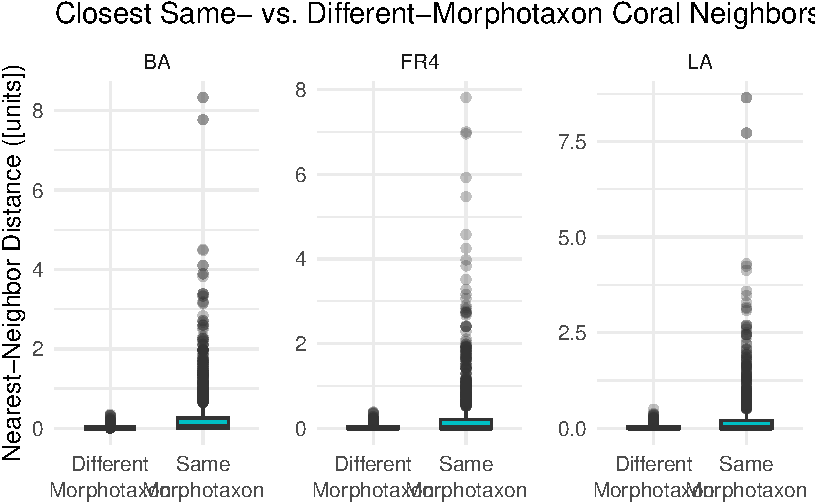
\includegraphics[keepaspectratio]{Coral_arcGIS_analysis_files/figure-pdf/fig-same-vs-diff-taxa-1.pdf}}

}

\caption{\label{fig-same-vs-diff-taxa}Distribution of closest
nearest-neighbor distances ({[}units{]}) to colonies of the same versus
different morphotaxon across reef sites (BA, FR4, and LA). A distance of
0 indicates touching or overlapping coral polygon boundaries; boxes show
the median and interquartile range (Q25--Q75), with whiskers extending
up to 1.5× IQR and points showing outliers.}

\end{figure}%

\begin{Shaded}
\begin{Highlighting}[]
\NormalTok{p\_ripley }\OtherTok{\textless{}{-}} \FunctionTok{ggplot}\NormalTok{(ripleys\_k, }\FunctionTok{aes}\NormalTok{(}\AttributeTok{x =}\NormalTok{ step)) }\SpecialCharTok{+}
  \FunctionTok{geom\_ribbon}\NormalTok{(}\FunctionTok{aes}\NormalTok{(}\AttributeTok{ymin =}\NormalTok{ LwConfEnv, }\AttributeTok{ymax =}\NormalTok{ HiConfEnv), }\AttributeTok{alpha =} \FloatTok{0.25}\NormalTok{, }\AttributeTok{fill =} \StringTok{"grey50"}\NormalTok{) }\SpecialCharTok{+}
  \FunctionTok{geom\_line}\NormalTok{(}\FunctionTok{aes}\NormalTok{(}\AttributeTok{y =}\NormalTok{ ExpectedK, }\AttributeTok{linetype =} \StringTok{"Expected K"}\NormalTok{), }\AttributeTok{linewidth =} \FloatTok{0.8}\NormalTok{) }\SpecialCharTok{+}
  \FunctionTok{geom\_line}\NormalTok{(}\FunctionTok{aes}\NormalTok{(}\AttributeTok{y =}\NormalTok{ ObservedK, }\AttributeTok{color =}\NormalTok{ site), }\AttributeTok{linewidth =} \DecValTok{1}\NormalTok{) }\SpecialCharTok{+}
  \FunctionTok{facet\_wrap}\NormalTok{(}\SpecialCharTok{\textasciitilde{}}\NormalTok{ site, }\AttributeTok{scales =} \StringTok{"free\_y"}\NormalTok{) }\SpecialCharTok{+}
  \FunctionTok{labs}\NormalTok{(}
    \AttributeTok{x =} \StringTok{"Distance Step"}\NormalTok{,}
    \AttributeTok{y =} \StringTok{"K Value"}\NormalTok{,}
    \AttributeTok{color =} \StringTok{"Site"}\NormalTok{,}
    \AttributeTok{linetype =} \ConstantTok{NULL}\NormalTok{,}
    \AttributeTok{title =} \StringTok{"Observed vs. Expected Ripley\textquotesingle{}s K and Confidence Envelope"}
\NormalTok{  ) }\SpecialCharTok{+}
  \FunctionTok{theme\_minimal}\NormalTok{(}\AttributeTok{base\_size =} \DecValTok{12}\NormalTok{) }\SpecialCharTok{+}
  \FunctionTok{theme}\NormalTok{(}\AttributeTok{panel.spacing =} \FunctionTok{unit}\NormalTok{(}\FloatTok{1.2}\NormalTok{, }\StringTok{"lines"}\NormalTok{))}

\FunctionTok{ggsave}\NormalTok{(}\StringTok{"outputs/fig\_ripleys\_k.png"}\NormalTok{, p\_ripley, }\AttributeTok{width =} \DecValTok{9}\NormalTok{, }\AttributeTok{height =} \DecValTok{5}\NormalTok{, }\AttributeTok{dpi =} \DecValTok{300}\NormalTok{)}
\NormalTok{p\_ripley}
\end{Highlighting}
\end{Shaded}

\begin{figure}[H]

\centering{

\pandocbounded{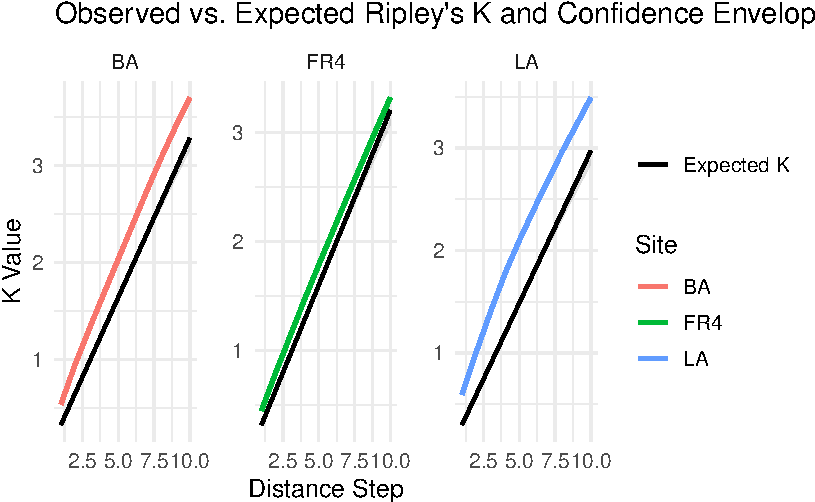
\includegraphics[keepaspectratio]{Coral_arcGIS_analysis_files/figure-pdf/fig-ripleys-k-1.pdf}}

}

\caption{\label{fig-ripleys-k}Multi-distance spatial clustering
(Ripley's K) across distance steps for each reef site. The shaded grey
band shows the simulation confidence envelope (LwConfEnv to HiConfEnv)
expected under complete spatial randomness; when ObservedK rises above
the upper confidence envelope, colonies are more spatially clustered
than random at that scale, whereas values inside or below the envelope
indicate random or dispersed spacing.}

\end{figure}%




\end{document}
